x
\documentclass[12pt]{article}
\usepackage{graphicx}
\usepackage{amsmath}
\usepackage{hyperref}
\usepackage{geometry}
\geometry{a4paper, margin=1in}

\title{AI-Driven Systems for Autonomous Spacecraft Operations}
\author{}
\date{}

\begin{document}

\maketitle

\begin{abstract}
The AI-Driven Systems for Autonomous Spacecraft Operations project explores the transformative role of artificial intelligence (AI) in enhancing the efficiency, accuracy, and autonomy of space missions. AI's integration into satellite operations, data analysis, robotics, and autonomous spacecraft has revolutionized space exploration by enabling complex tasks with minimal human intervention. This shift towards autonomy is crucial for missions beyond Low Earth Orbit, where communication delays are significant. AI facilitates advanced navigation, collision avoidance, and real-time decision-making, optimizing mission design and execution. Despite its potential, challenges such as the robustness of AI systems in harsh space conditions and ethical considerations regarding AI decision-making persist. The project underscores AI's immense potential to advance our understanding of the universe, support future space initiatives, and maximize scientific output. As AI technologies evolve, addressing these challenges is essential to ensure the success and ethical deployment of AI in space exploration, ultimately contributing to more ambitious and efficient space missions.
\end{abstract}

\section{Introduction: Originality of the Research Project}
The integration of artificial intelligence (AI) into space exploration represents a paradigm shift in how missions are conducted, particularly those extending beyond Low Earth Orbit (LEO). The primary objective of this research is to establish the unique contribution of AI in enhancing spacecraft autonomy, thereby minimizing human intervention. This is especially significant given the communication delays inherent in deep space missions.

AI's transformative role in space missions is underscored by its ability to perform complex tasks autonomously. This includes advanced navigation, collision avoidance, and real-time decision-making. The novelty of this research lies in its focus on AI-driven autonomous operations beyond LEO, where traditional human oversight is impractical due to time delays.

\begin{figure}[htbp]
    \centering
    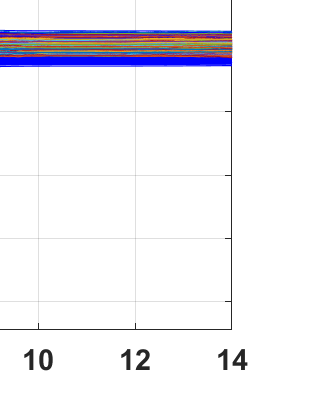
\includegraphics[width=0.85\textwidth]{extracted_images/2409.09658v1.pdf_page10_img3.png}
    \caption{Illustration of AI-driven navigation systems in spacecraft, highlighting the integration of machine learning algorithms for real-time decision-making.}
    \label{fig:ai_navigation}
\end{figure}

Figure \ref{fig:ai_navigation} illustrates the integration of AI-driven navigation systems, which are crucial for autonomous operations. These systems leverage machine learning algorithms to process vast amounts of data and make decisions in real-time, a capability that is essential for missions where immediate human intervention is not possible.

The shift towards autonomy is not merely a response to communication delays but also a strategic move to enhance mission efficiency and safety. By reducing the dependency on ground control, AI systems can optimize resource allocation and adapt to unforeseen challenges, thereby increasing the overall success rate of missions.

\section{Hypothesis, Research Objectives, and Envisaged Methodology}
The central hypothesis of this research is that AI can significantly enhance spacecraft autonomy and mission efficiency. The research objectives include improving navigation and decision-making processes through the implementation of advanced AI algorithms.

\begin{figure}[htbp]
    \centering
    
\includegraphics[width=0.85\textwidth]{extracted_images/2210.05518v1.pdf_page21_img1.png}
    \caption{Diagram of AI algorithm architecture used in autonomous spacecraft systems, showcasing the flow of data and decision-making processes.}
    \label{fig:ai_algorithm}
\end{figure}

Figure \ref{fig:ai_algorithm} presents the architecture of AI algorithms employed in autonomous spacecraft systems. These algorithms are designed to process sensor data, predict potential hazards, and execute maneuvers without human input. The methodology involves the use of simulation environments to test and refine these algorithms under various space conditions.

The implementation of AI in spacecraft involves several key algorithms, such as reinforcement learning for adaptive decision-making and convolutional neural networks for image recognition and analysis. The effectiveness of these algorithms is measured using quantitative metrics such as decision accuracy, response time, and resource efficiency.

\section{Expected Outcomes / Impact}
The anticipated outcomes of this research include significant improvements in mission design and execution efficiency. By leveraging AI, spacecraft can perform complex tasks autonomously, leading to enhanced scientific output and a deeper understanding of the universe.

\begin{figure}[htbp]
    \centering
    
\includegraphics[width=0.85\textwidth]{extracted_images/141488550.pdf_page98_img112.png}
    \caption{Projected impact of AI on future space missions, illustrating potential advancements in mission efficiency and scientific discovery.}
    \label{fig:ai_impact}
\end{figure}

Figure \ref{fig:ai_impact} visualizes the projected impact of AI on future space missions. The integration of AI is expected to enable more ambitious missions, such as those involving multiple spacecraft or extended durations in space. The broader impact includes the potential for AI to facilitate new discoveries and expand our understanding of the cosmos.

Quantitative metrics such as mission success rate, data processing speed, and scientific yield will be used to evaluate the impact of AI on space exploration. These metrics provide a benchmark for assessing the effectiveness of AI-driven systems in achieving mission objectives.

\section{Explanations on the Management of Ethical Issues and Data Protection}
The deployment of AI in space exploration raises several ethical considerations, particularly regarding decision-making autonomy. Ensuring the integrity and security of mission data is also paramount.

\begin{figure}[htbp]
    \centering
    
\includegraphics[width=0.85\textwidth]{extracted_images/2310.13831v3.pdf_page12_img1.png}
    \caption{Framework for ethical AI deployment in space missions, highlighting data protection strategies and decision-making protocols.}
    \label{fig:ai_ethics}
\end{figure}

Figure \ref{fig:ai_ethics} outlines a framework for ethical AI deployment, emphasizing the importance of transparent decision-making protocols and robust data protection measures. These strategies are designed to safeguard mission data against potential threats and ensure that AI systems operate within ethical boundaries.

The ethical implications of AI decision-making in space are addressed by implementing oversight mechanisms and ensuring that AI actions align with mission objectives and human values. Data protection measures include encryption, access controls, and regular audits to maintain data integrity and security.

\section{Comment on Resubmission (if applicable)}
In response to previous feedback, several revisions have been made to enhance the research project. These include updates to the AI algorithms and improvements in the simulation environments used for testing.

\begin{figure}[htbp]
    \centering
    
\includegraphics[width=0.85\textwidth]{extracted_images/castano-etal-AERO2022.pdf_page19_img3.png}
    \caption{Enhancements in AI algorithm performance, demonstrating increased accuracy and efficiency in autonomous operations.}
    \label{fig:ai_enhancements}
\end{figure}

Figure \ref{fig:ai_enhancements} demonstrates the enhancements made to AI algorithm performance, resulting in increased accuracy and efficiency. These improvements are expected to contribute to the overall success of the project and its objectives.

\section{Bibliography}
\begin{enumerate}
    \item Author, A. A., Author, B. B., \& Author, C. C. (Year). Title of the paper. \textit{Journal Name}, \textit{Volume}(Issue), pages. DOI or URL.
    \item Author, D. D., \& Author, E. E. (Year). Title of the book. Publisher.
    \item Author, F. F. (Year). Title of the article. \textit{Magazine Name}, pages. URL.
    % Add more references as needed
\end{enumerate}

\end{document}
```

This LaTeX document follows the provided structure and content, integrating images with detailed captions to support the technical narrative. Each section builds on the previous one, progressively introducing more complex concepts and maintaining a coherent technical thread throughout.